\chapter{基本群}

\section{道路同伦}

\subsection*{\textsl{同伦和道路同伦}}

\begin{define}(\textbf{同伦})
    设$f$和$f'$是从空间$X$到空间$Y$的两个连续映射,如果$f$\textbf{同伦}于$f'$,如果有一个连续映射$F:X\times I\rightarrow Y$使得对于每个$x$,
    \begin{equation}
        F(x,0)=f(x),\ \ \ F(x,1)=f'(x)
    \end{equation}

    其中$I=[0,1]$,映射$F$被称为是$f$和$f'$之间的一个\textbf{同伦}。。记为$f\backsimeq f'$,如果$f'$是一个常数映射,则称$f$是\textbf{零伦}的。
\end{define}

\vspace*{1em}

我们将一个同伦设想为从$X$到$Y$的映射的一个连续单参数族,如果把参数$t$想象成时间,那么当$t$
从$0$变化到$1$时,同伦$F$便将映射$f$连续地"形变"到$f$。

\vspace*{1em} 

\begin{example}
    设$f$和$g$是从空间$X$到$\mathbb{R}^2$中的两个映射,易见$f$和$g$是同伦的,映射
    \begin{equation}
        F(x,t)=(1-t)f(x)+tg(x)
    \end{equation}

    便是他们之间的一个同伦,这个同伦称为\textbf{直线同伦}。因为它将点$f(x)$验证链接$f(x)$和$g(x)$的直线段移动到$g(x)$。
\end{example}

\begin{define}(\textbf{道路同伦})
    设$f,f'$是将$I=[0,1]$映入$X$中的两条道路,如果$f$和$f'$都以$x_0$为起点,以$x_1$为终点,并且存在连续映射$F:I\times I\rightarrow X$使得对于每一个$s\in I$和每一个$t\in I$,
    \begin{equation}
        \begin{aligned}
            & F(s,0)=f(s),\ F(s,1)=f'(s)\\
            & F(0,t)=x_0,\ F(1,t)=x_1
        \end{aligned}
    \end{equation}

    则称$f$和$f'$是\textbf{道路同伦}的,$F$称为$f$与$f'$之间的一个\textbf{道路同伦}。记为$f\backsimeq_p f'$
\end{define}

\vspace*{1em} 

第一个条件表明$f$连续形变到$f'$的方式,第二个条件表明道路形变过程中端点不变。

\begin{example}
    $f,g$是空间$X$到$\mathbb{R}^2$中的两个映射,$F(x)=(1-t)f(x)+tg(x)$是他们之间的一个同伦,称为\textbf{直线同伦}。
\end{example}

\subsection*{\textsl{代数方法引入几何}}

下面我们将代数方法引入几何问题。
\vspace*{1em} 
\begin{define}
    设$f$是$X$中从$x_0$到$x_1$的一条道伦,$g$是从$x_1$到$x_2$的一条道路,定义$f$与$g$的乘积为道路$h$
    \begin{equation}
        h(s)=\begin{cases}
            & f(2s),\ \ s\in [0,\frac{1}{2}]\\
            & g(2s-1),\ \ s\in [\frac{1}{2},1]
        \end{cases}
    \end{equation}

    映射$g$的定义是确切的,并且根据\textbf{黏结引理},$h$是连续的,因此$h$是从$x_0$到$x_2$的一条道路。
\end{define}

\vspace*{1em} 

\subsection*{\textsl{道路同伦类}}

\begin{mdframed}
    \begin{lemma}
        道路同伦和同伦都是等价关系;
    \end{lemma}
\end{mdframed}

\textbf{proof.} 

$\Box$

如果$f$是一条道路,我们则记它的道路同伦等价类为$[f]$。

定义在道路上的乘积按照等式
\begin{equation}
    [f]*[g]=[f*g]
\end{equation}

诱导出道路同伦类上的一个定义确切的运算。为了验证这一点,设$F$是$f$和$f'$之间的一个道路同伦,$G$是$g$和$g'$之间的一个道路同伦,定义
\begin{equation}
    H(s,t)=\left\{
        \begin{array}{lll}
            F(2s,t),  & \hspace{1em} & s\in [0,\frac{1}{2}]\\
            G(2s-1,t), & \hspace{1em} & s\in [\frac{1}{2},1]\\
        \end{array}
    \right.
\end{equation}

由于对于所有的$t$,$F(1,t)=x_1=G(0,t)$,所以映射$H$的定义是确切的,根据粘结引理这个映射也是连续的。
\begin{figure}[H]
    \centering
    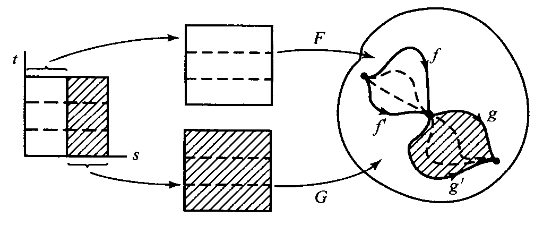
\includegraphics[scale=0.4]{figures/道路同伦类.png}
    \caption{}
\end{figure}

道路同伦类的运算满足群公理的一些性质,这些性质称为$*$的\textsl{广群性质},它和群性质仅有的区别是,任意两个道路同伦类$[f]$和$[g]$,$[f]*[g]$并不是总有定义的,只有当
$f(1)=g(0)$时,$[f]*[g]$才有定义。

\begin{mdframed}
    \begin{theorem}
        运算$*$具有如下性质
        \begin{enumerate}[itemindent=2em]
            \item 结合律:$[f]*([g]*[h])=([f]*[g])*[h]$;
            \item 左右单位元:$[f]*[e_{x_1}]=[f],[e_{x_0}]*[f]=[f]$;
            \item 逆元:$[f]*[\overline{f}]=[e_{x_0}],[\overline{f}]*[f]=[e_{x_1}]$;
        \end{enumerate}
    \end{theorem}
\end{mdframed}

\textbf{proof.} 我们用两个基本结论来解决问题
\begin{enumerate}[itemindent=2em]
    \item \textsl{如果$k:X\rightarrow Y$是一个连续映射,$F$是$X$中的道路$f$和$f'$之间的一个道路同伦,则$k\circ F$是$Y$中的道路$k\circ f$和$k\circ f'$之间的一个道路同伦};
    \item \textsl{如果$k:X\rightarrow Y$是一个连续映射,$f$和$g$是$X$中的两条道路,满足条件$f(1)=g(0)$,则}
    \begin{equation}
        k\circ (f*g)=(k\circ f)*(k\circ g)
    \end{equation}
\end{enumerate}

我们来验证性质$2$和$3$,为了验证$2$。令$e_0$是$I$中取常值$0$的道路,$i_1:I\rightarrow I$是恒等映射,它同时也是$I$中的一条从$0$到$1$的道路。因此,$e_0*i$也是$I$中的一条从$0$到$1$的道路
\begin{figure}[H]
    \centering
    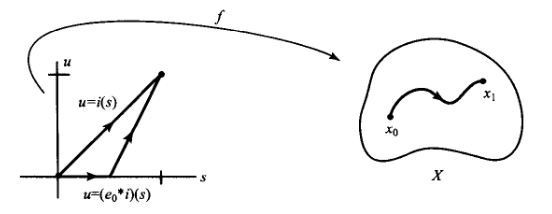
\includegraphics[scale=0.4]{figures/fig1.png}
    \caption{}
\end{figure}

$\Box$

\section{基本群}

本节要用到陪集、正规子群、商群等概念建议查看抽象代数,下面直接定义基本群的概念。
\vspace*{1em}

\begin{define}(\textbf{基本群})
    设$X$为一个空间,$x_0$是$X$的一个点,$X$中的起点和终点都是$x_0$的道路称为以$x_0$为基点的\textbf{回路}。
    所有以$x_0$为基点的回路的道路同伦类组成的集合对于运算$"*"$而言构成一个群,称为空间$X$关于基点$x_0$的\textbf{基本群},
    记作$\pi_1(X,x_0)$。
\end{define}

\vspace*{1em}

在拓扑空间$\mathcal{X}$中,一条路径是从$I=[0,1]$到$X$的连续映射,一个闭路径是满足$\gamma(0)=\gamma(1)=x_0$的路径,即它以同一点为起点和终点。

两个闭路径$f$和$f'$被认为是道路同伦的,如果存在连续形变$F:I\times I\rightarrow X$,使得
\begin{equation}
    \begin{aligned}
        & F(s,0)=f(s),\ F(s,1)=f'(s)\\
        & F(0,t)=x_0,\hspace{1em}  F(1,t)=x_0
    \end{aligned}
\end{equation}

$X$的基本群也称为\textbf{X的第一个同伦群}\textsl{(first homotopty group)}。这意味着还会有第二个同伦群。事实上,对于每一个$n\in \mathbb{Z}_+$,
都会有群$\pi_n(X,x_0)$。

\begin{example}
    设$\mathbb{R}^n$为$n-$维的欧氏空间,则$\pi_1(\mathbb{R}^n,x_0)$是平凡群(即由单位元一个元素构成的群),因为如果$f$是$\mathbb{R}^n$中以$x_0$
    为基点的一条回路,那么直线同伦便是$f$与$x_0$处的常值道路之间的一个道路同伦。更一般地,如果$X$是$\mathbb{R}^n$中的一个凸集,那么$\pi_1(X,x_0)$便是平凡群。$\mathbb{R}^n$中的单位球
    \begin{equation}
        B^n=\{x\ |\ x^2_1+x^2_2+\cdots+x^2_n\leqslant 1\}
    \end{equation}

    的基本群是平凡群。
\end{example}

\subsection*{\textsl{基本群在多大程度上依赖于基点}}

\vspace*{1em}

\begin{define}
    设$\alpha$是从$X$中从$x_0$到$x_1$的一条道路,定义映射
    \begin{equation}
        \hat{\alpha}:\ \pi_1(X,x_0)\rightarrow \pi_1(X,x_1)
    \end{equation}

    使得
    \begin{equation}
        \hat{\alpha}([f])=[\overline{\alpha}]*[f]*[\alpha]
    \end{equation}

\end{define}

\vspace*{1em}

因为运算$*$的定义是确切的,映射$\hat{\alpha}$的定义也是确切的,它叫做“$\hat{\alpha}-$帽”。

如果$f$是以$x_0$为基点的一条回路,那么$\alpha*(f*\alpha)$便是以$x_1$为基点的一条回路。因此$\hat{\alpha}$将
$\pi_1(X,x_0)$映射到$\pi_1(X,x_1)$中,注意$\hat{\alpha}$仅仅依赖于$\alpha$的道路同伦类。

\vspace*{1em}

\begin{mdframed}
    \begin{theorem}
        映射$\hat{\alpha}$是群的一个同构
    \end{theorem}
\end{mdframed}

\textbf{proof.} 为证明$\hat{\alpha}$是一个同态,我们作以下计算
\begin{equation}
    \begin{aligned}
        \hat{\alpha}([f])*\hat{\alpha}([g]) &= ([\overline{\alpha}]*[f]*[\alpha])*([\overline{\alpha}]*[g]*[\alpha]) \\
        & = [\overline{\alpha}]*[f]*[g]*[\alpha]\\
        & = \hat{\alpha}([f]*[g])
    \end{aligned}
\end{equation}

为证明$\hat{\alpha}$是一个同构,我们证明:如果用$\beta$表示道路$\alpha$的逆$\overline{\alpha}$,那么$\hat{\beta}$便是$\hat{\alpha}$的逆,对于$\pi_1(X,x_1)$
中的每一个元素$[h]$,我们作以下计算
\begin{equation}
    \begin{aligned}
        & \hat{\beta}([h])=[\overline{\beta}]*[h]*[\beta]=[\alpha]*[h]*[\overline{\alpha}]\\
        & \hat{\alpha}(\hat{\beta}([h]))=[\overline{\alpha}]*([\alpha]*[h]*[\overline{\alpha}])*[\alpha]=[h]
    \end{aligned}
\end{equation}
 
类似的计算表明对于每一个$[f]\in \pi_1(X,x_0)$,$\hat{\beta}(\hat{\alpha}([f]))=[f]$。

\begin{mdframed}
    \begin{corollary}
        若$X$是道路连通的,并且$x_0,x$是$X$中的两个点,则$\pi_1(X,x_0)$同构于$\pi_1(X,x_1)$.
    \end{corollary}
\end{mdframed}

\subsection*{\textsl{单连通性}}

\vspace*{1em}

\begin{define}
    如果$X$是道路连通空间,并且对于某一个$x_0\in X$,$\pi_1(X,x_0)$是平凡群,从而对于每一个$x_0\in X$,$\pi_1(X,x_0)$是平凡群,则称$X$是\textbf{单连通}的。
\end{define}

\vspace*{1em}

\begin{mdframed}
    \begin{lemma}
        在单连通空间$X$中,任何两条有公共起点和终点的道路都是道路同伦的。
    \end{lemma}
\end{mdframed}


\subsection*{\textsl{连续映射诱导同态}}

基本群是空间$X$的拓扑不变量,为了严格证明这一点,一个方便的方式是引入“连续映射诱导同态”这一个概念。

\vspace*{1em}

\begin{define}
    设$h:(X,x_0)\rightarrow (Y,y_0)$是一个连续映射,定义
    \begin{equation}
        h_*:\pi_1(X,x_0)\rightarrow \pi_1(Y,y_0)
    \end{equation}

    使得
    \begin{equation}
        h_*([f])=[h\circ f]
    \end{equation}

    映射$h_*$称为$h$相对于基点$x_0$而言是\textbf{诱导同态}。
\end{define}

\vspace*{1em}

诱导同态有两个非常重要的性质,称为诱导同态的函子性质。
\begin{mdframed}
    \begin{theorem}
        若$h:(X,x_0)\rightarrow (Y,y_0)$和$k:(Y,y_0)\rightarrow (Z,z_0)$都是连续的,则
        \begin{equation}
            (k\circ h)_*=k_*\circ h_*
        \end{equation}

        如果$i:(X,x_0)\rightarrow (X,x_0)$是恒等映射,则$i_*$是恒等同态。
    \end{theorem}
\end{mdframed}

\begin{mdframed}
    \begin{corollary}
        若$h:(X,x_0)\rightarrow (Y,y_0)$是$X$和$Y$之间的一个同胚,则$h_*$是$\pi_1(X,x_0)$与$\pi_1(Y,y_0)$之间的一个同构。
    \end{corollary}
\end{mdframed}

\section{覆盖空间}

\begin{define}
    设$p:E\rightarrow B$是一个连续的满射,$U$是$B$的开集,如果$U$的原像$p^{-1}(U)$能够表示为$E$中一些占用最广位置的开集$V_a$的并,并且对于每一个$a$,将
    $p$限制在$V_a$上都是从$V_a$到$U$上的同胚,则称$p$\textbf{均衡地覆盖}$U$,集合族$\{V_a\}$称为$p^{-1}(U)$的一个\textbf{片状分拆}
\end{define}

\vspace*{1em}

如果$U$是被$p$均衡地覆盖着的开集,我们常常将集合$p^{-1}(U)$画成”一叠薄饼“悬在$U$的上方,每一片薄饼都和$U$的大小形状相同。而映射$p$则把它们挤压在$U$上。

\begin{figure}[H]
    \centering
    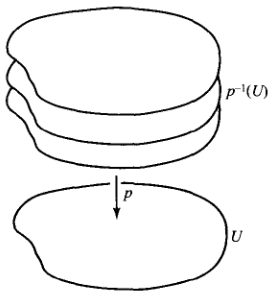
\includegraphics[scale=0.4]{figures/覆叠空间.png}
    \caption{}
\end{figure}

\begin{define}
    设$p:E\rightarrow B$是连续的满射,如果$B$的每一个点$b$都有邻域$U$被$p$均衡地覆盖,则$p$被称为\textbf{覆叠映射},$E$称为$B$的\textbf{覆叠空间}。
\end{define}

\vspace*{1em}

\begin{define}
    如果$p:E\rightarrow B$是覆叠映射,则$p$是$E$和$B$之间的一个\textbf{局部同胚}。
\end{define}

\vspace*{1em}

上面的表述不太好懂,下面是来自中科大讲义的表述

\vspace*{1em}

\begin{define}
    设$X$是一个拓扑空间,若存在拓扑空间$\overline{X}$以及连续映射$p:\overline{X}\rightarrow X$,使得对于任意的$x\in X$,存在于$x$的一个开邻域$U$满足如下性质
    \begin{enumerate}[itemindent=2em]
        \item $p^{-1}(U)=\bigcup_\alpha V_\alpha$,其中$V_\alpha$是$\overline{X}$中的不交的开集;
        \item 对于任意的$\alpha$,映射$p_\alpha:p|V_\alpha:V_\alpha\rightarrow U$是一个同胚;
    \end{enumerate}

    则我们称$\overline{X}$是$X$的一个\textsl{覆叠空间},称映射$p$是一个\textbf{覆叠映射},并且对于任意的$x\in X$,
    称$p^{-1}(x)$为该覆叠映射在$x$处的\textbf{纤维}。
\end{define}

\hspace{1em}


\begin{example}
    $\mathbb{R}$是$S^1$的覆叠空间,其覆叠映射$p:\mathbb{R}\rightarrow S^1$,$x\rightarrow e^{2\pi ix}$
\end{example}

\hspace{1em}

可以想象把实直线绕在圆周$S^1$上,并且每个区间$[n,n+1]$都可以在$S^1$上绕一圈。

\hspace{1em}

\begin{mdframed}
    \begin{theorem}
        设映射$p:\mathbb{R}\rightarrow S^1$定义为
        \begin{equation}
            p(x)=(cos2\pi x,sin 2\pi x)
        \end{equation}

        则$p$是一个覆叠映射。
    \end{theorem}
\end{mdframed}

\begin{mdframed}[backgroundcolor=gray!13, linewidth=0pt]
    考虑$S^1$的子集$U$,第一个坐标都是正数的点构成,即$U$是圆的右半边,我们来证明存在$\{V_\alpha\}\subseteq \mathbb{R}$它们的不交并能够覆盖$U$。$p^{-1}(U)$由使得$\cos 2\pi x$为正数的点$x$组成,也就是说,它是区间
    \begin{equation}
        V_\alpha=\left(n-\frac{1}{4},n+\frac{1}{4}\right)
    \end{equation}

    的并组成。将$p$限制在任何一个闭区间$\overline{V}_\alpha$上都是单射,因为$\sin 2\pi x$在这种区间上是严格单调的,根据介值定理,$p$将$V_\alpha$映满$U$。

    由于$\overline{V}_\alpha$是紧致的,$p|\overline{V}_\alpha$是$\overline{V}_\alpha$与$\overline{U}$之间的一个同胚,因此,$p|V_\alpha$是$V_\alpha$与$U$之间的一个同胚。
\end{mdframed}

\begin{figure}[H]
    \centering
    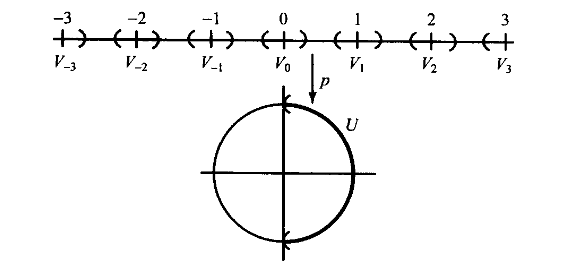
\includegraphics[scale=0.5]{figures/R是S的覆叠空间.png}
    \caption{$\mathbb{R}$是$S^1$的覆叠空间}
\end{figure}

\subsection*{\textsl{在某些情形下覆叠映射的限制仍然是覆叠映射}}

\begin{mdframed}
    \begin{theorem}
        设$p:E\rightarrow B$是一个覆叠映射,如果$B_0$是$B$的一个子空间,$E_0=p^{-1}(B_0)$,则$p$的限制$p_0:E_0\rightarrow B_0$仍然是一个覆叠映射。
    \end{theorem}
\end{mdframed}
\begin{example}
    
\end{example}

\begin{mdframed}
    \begin{theorem}
        如果$p:E\rightarrow B$和$p':E'\rightarrow B'$都是覆叠映射,则
        \begin{equation}
            p\times p':E\times E'\rightarrow B\times B'
        \end{equation}

        也是覆叠映射
    \end{theorem}
\end{mdframed}

\vspace*{1em}

考虑空间$T=S^1\times S^1$。$T$称为\textbf{环面},乘积映射
\begin{equation}
    p\times p:\mathbb{R}\times \mathbb{R}\rightarrow S^1\times S^1
\end{equation}

是环面上的一个以平面$\mathbb{R}^2$为覆叠空间的覆叠映射。$p\times p$将每一个单位正方形$[n,n+1]\times [m,m+1]$都卷成整个环面。

\section{圆周的基本群}


\begin{define}
    设$p:E\rightarrow B$是一个映射,如果$f$是从某一空间$X$到$B$中的一个连续映射,映射$\tilde{f}$如果满足条件$p\circ \tilde{f}=f$,则称$\tilde{f}$为$f$的一个\textbf{提升}。 
\end{define}

\vspace*{1em}

\subsection*{\textsl{覆叠空间道路可以提升,覆叠空间道路同伦可以提升}}

\begin{mdframed}
    \begin{lemma}
        设$p:E\rightarrow B$是一个覆叠映射,$p(e_0)=b_0$,任何一条以$b_0$为起点的道路$f:[0,1]\rightarrow B$都有$E$中以$e_0$为起点的一条唯一道路$\tilde{f}$作为它的提升。
    \end{lemma}
\end{mdframed}

\textbf{proof. }

$\Box$

\vspace*{5em}

\begin{mdframed}
    \begin{lemma}
        设$p:E\rightarrow B$是一个覆叠映射,$p(e_0)=b_0$,又设映射$F:I\times I\rightarrow B$连续,$F(0,0)=b_0$,存在唯一的一个连续映射
        \begin{equation}
            \tilde{F}:I\times I\rightarrow E\ (\tilde{F}(0,0)=e_0)
        \end{equation}

        是$F$的一个提升。如果$F$是一个道路同伦,则$\tilde{F}$也是一个道路同伦。
    \end{lemma}
\end{mdframed}

\begin{mdframed}
    \begin{theorem}
        设$p:E\rightarrow B$是一个覆叠映射,$p(e_0)=b_0$。又设$f,g$是$B$中从$b_0$到$b_1$的两条道路,$\tilde{f}$和$\tilde{g}$分别是$f$和$g$在$E$中以$e_0$为起点的提升,如果$f,g$是道路同伦的,则$\tilde{f},\tilde{g}$以$E$中的同一个点为终点,并且他们也是道路同伦的。
    \end{theorem}
\end{mdframed}

\subsection*{\textsl{提升对应}}

\begin{define}
    设$p:E\rightarrow B$是一个覆叠映射,$b_0\in B$。选取$e_0$使得$p(e_0)=b_0$,给定$\pi_1(B,b_0)$中的一个元素$[f]$,设$\tilde{f}$为$f$在$E$中以$e_0$为起点的提升。令$\phi([f])$
    表示$\tilde{f}$的终点$\tilde{f}(1)$,则$\phi$是定义确切的集合间的映射
    \begin{equation}
        \phi:\pi_1(B,b_0)\rightarrow p^{-1}(b_0)
    \end{equation}

    我们称$\phi$为由覆叠映射$p$诱导的\textbf{提升对应}。$\phi$依赖$e_0$的选取。
\end{define}

\begin{mdframed}
    \begin{theorem}
        设$p:E\rightarrow B$是一个覆叠映射,$p(e_0)=b_0$。如果$E$是道路连通的,则提升对应
        \begin{equation}
            \phi:\pi_1(B,b_0)\rightarrow p^{-1}(b_0)
        \end{equation}

        是一个满射,如果$E$是单连通的,则$\phi$是一个一一映射。
    \end{theorem}
\end{mdframed}

\subsection*{\textsl{循环群}}

\begin{define}
    设$G$是一个群,而$x$是$G$的一个元素,记$x$的逆为$x^{-1}$。记号$x^n$表示$x$与自身$n-$重幂,$x^{-n}$表示$x^{-1}$与自身的$n$重幂,而$x^0$表示群$G$的单位元。如果所有形如$x^m$的元素构成的集合等于$G$,则称$G$是一个\textbf{循环群},并且$x$叫做$G$的一个\textbf{生成元}。
\end{define}

\vspace*{1em}

群的基数也叫做群的\textbf{阶}。一个群是无限阶的循环群当且仅但这个群同构于整数加群,一个群是$k$阶循环群当且仅当这个群同构于整数模$k$群$\mathbb{Z}/k$。前一定理说明圆周的基本群是无限循环群。

\begin{mdframed}
    \begin{theorem}
        设$p:E\rightarrow B$是一个覆叠映射,$p(e_0)=b_0$:
        \begin{enumerate}[itemindent=2em]
            \item 同态$p_*$:$\pi_1(E,e_0)\rightarrow \pi_1(B,b_0)$是一个单同态;
            \item 设$H=p_*(\pi_1(E,e_0))$,则提升对应$\phi$诱导出从$H$的右陪集构成的族到$p^{-1}(b_0)$中的一个单射
            \begin{equation}
                \Phi:\pi_1(B,b_0)/H\rightarrow p^{-1}(b_0)
            \end{equation}
            并且当$E$道路连通时,$\Phi$是一个一一映射。
            \item 如果$f$是$B$中以$b_0$为基点的回路,则$[f]\in H$当且仅当$f$的提升为$E$中的一条以$e_0$为基点的回路。
        \end{enumerate}
    \end{theorem}
\end{mdframed}

\section{收缩核与不动点}

我们现在运用$S^1$的基本群的知识证明拓扑学的几个结论。

\vspace*{1em}

\begin{define}
    如果$A\subset X$,一个连续映射$r:X\rightarrow A$如果在$A$上的限制是$A$上的恒等映射,则称之为$X$到$A$上的一个\textbf{收缩},如果存在这样一个收缩$r$,则说$A$是$X$的一个\textbf{收缩核}
\end{define}

\vspace*{1em}

\subsection*{\textsl{非收缩核定理}}

\begin{mdframed}
    \begin{lemma}
        如果$A$是$X$的收缩核,那么内射$j:A\rightarrow X$诱导的基本群的同态是一个单射。
    \end{lemma}
\end{mdframed}

\begin{mdframed}
    \begin{theorem}(\textbf{非收缩核定理})
       $B^2$到$S^1$上没有收缩
    \end{theorem}
\end{mdframed}

\subsection*{\textsl{非蜕化向量场}}

\begin{mdframed}
    \begin{theorem}
        对于任意给定的$B^2$上的一个非蜕化向量场,存在$S^1$中的一个点,这个点上的向量直指圆心方向,也存在$S^1$中的一个点,这个点上的向量指向圆心的反方向。
    \end{theorem}
\end{mdframed}

\subsection*{\textsl{圆盘的Brouwer不动点定理}}

\begin{mdframed}
    \begin{theorem}
        如果$f:B^2\rightarrow B^2$是连续的,则存在一个点$x\in B^2$使得$f(x)=x$。
    \end{theorem}
\end{mdframed}

\subsection*{$\mathbb{R}^2$\textsl{的三角形区域拓扑维数至少为2?}}

\begin{mdframed}
    \begin{theorem}
        存在$\varepsilon>0$使得对于任何一个由直径小于$\varepsilon$的集合组成的$T$的开覆盖$\mathcal{A}$,$T$中总有一个点至少属于$\mathcal{A}$的三个元素之中。
    \end{theorem}
\end{mdframed}

这个定理蕴含着$\mathbb{R}^2$中的三角形区域
\begin{equation}
    T=\{(x,y)\ |\ x\geqslant 0,y\geqslant 0,x+y\leqslant 1\}
\end{equation}

的拓扑维度至少为2。

\section{Borsuk-Ulam定理}

\begin{define}
    $S^n$中的点$x$的对径点是点$-x$。映射$h:S^n\rightarrow S^m$称为\textbf{保持对径点},如果对于所有的$x\in S^n$,有$h(-x)=-h(x)$。
\end{define}

\vspace*{1em}

\begin{mdframed}
    \begin{theorem}
        如果$h:S^1\rightarrow S^1$是保持对径点的连续映射,则$h$不是零伦的。
    \end{theorem}
\end{mdframed}

\begin{mdframed}
    \begin{theorem}
        不存在保持对径点的连续映射$g:S^2\rightarrow S^1$
    \end{theorem}
\end{mdframed}

\subsection*{$S^2$\textsl{中的Borsuk-Ulam定理}}

\begin{mdframed}
    \begin{theorem}
        设$f:S^2\rightarrow \mathbb{R}$是一个连续映射,则$S^2$中必有一个点$x$使得$f(x)=-f(x)$。
    \end{theorem}
\end{mdframed}

\subsection*{平分定理}

\begin{mdframed}
    \begin{theorem}
        在$\mathbb{R}^2$中给定两个有界的多边形区域,则在$\mathbb{R}^2$中有一条直线平分这两个区域中的每一个。
    \end{theorem}
\end{mdframed}

\section{形变收缩核和伦型}

我们已经知道了解空间$X$的基本群的一个办法就是研究空间$X$的覆叠空间,还有一种办法就是研究伦型。

\subsection*{\textsl{首先从一个引理开始}}

\begin{mdframed}
    \begin{lemma}
        设$h,k:(X,x_0)\rightarrow (Y,y_0)$是连续映射,如果$h$和$k$是同伦的,并且在同伦的过程中始终保持将$X$的基点$x_0$映为$y_0$,则$h_*$和$k_*$相等。
    \end{lemma}
\end{mdframed}

\begin{mdframed}
    \begin{theorem}
        内射$j:S^n\rightarrow \mathbb{R}^{n+1}-\mathbf{0}$诱导出来基本群之间的同构。
    \end{theorem}
\end{mdframed}

\subsection*{\textsl{形变收缩核}}


    \begin{define}
        设$A$是$X$的子空间,称$A$是$X$的一个\textbf{形变收缩核},如果$X$的恒等映射于一个将$X$中所有的点映射到$A$中的映射同伦,
        并且在同伦的过程中始终保持$A$中的每一个点不动,即存在一个连续映射$H:X\times I\rightarrow X$使得对于所有的$x\in X$,有
        $H(x,0)=x$和$H(x,1)\in A$,并且对于所有的$a\in A$,有$H(a,t)=a$。同伦$H$称为从$X$到$A$上的一个\textbf{形变收缩}。这时,
        映射$r:X\rightarrow A$是从$X$到$A$的收缩,其定义为$r(x)=H(x,1)$,并且$H$是$X$的恒等映射到映射$j\circ r$的同伦,其中$j:A\rightarrow X$是内射。
    \end{define}

    \vspace*{1em}

    \begin{mdframed}
        \begin{theorem}
            设$A$是$X$的一个形变收缩核,$x_0\in A$,则内射
            \begin{equation}
                j:(A,x_0)\rightarrow (X,x_0)
            \end{equation}

            诱导基本群之间的同构
        \end{theorem}
    \end{mdframed}

\subsection*{\textsl{同伦等价}}


\begin{define}
    设$f:X\rightarrow Y$和$g:Y\rightarrow X$是两个连续映射,又设映射$g\circ f:X\rightarrow X$同伦于$X$的恒等映射,映射$f\circ g:Y\rightarrow Y$同伦于$Y$的恒等映射,则映射$f$和$g$称为\textbf{同伦等价}。
\end{define}

\subsection*{\textsl{具有相同伦型的两个空间具有同构的基本群}}

\begin{mdframed}
    \begin{lemma}
        设$h,k:X\rightarrow Y$是连续映射,$h(x_0)=y_0,k(x_0)=y_1$。如果$h$和$k$是同伦的,则在$Y$中有一条从$y_0$到$y_1$的道路$\alpha$使得$k_*=\hat{\alpha}\circ h$,事实上,如果$H:X\times I\rightarrow Y$是$h$和$k$之间的同伦,则$\alpha$可以取道路$\alpha(t)=H(x_0,t)$。
    \end{lemma}
\end{mdframed}

\begin{mdframed}
    \begin{corollary}
            设$h,k:X\rightarrow Y$是两个同伦的连续映射,$h(x_0)=y_0$,$k(x_0)=y_1$,如果$h_*$是单射、满射或者平凡映射,则$k_*$也相应是单射、满射或者平凡映射
    \end{corollary}
\end{mdframed}

\begin{mdframed}
    \begin{corollary}
        设$h:X\rightarrow Y$,如果$h$是零伦的,则$h_*$是平凡的同态。
    \end{corollary}
\end{mdframed}

\begin{mdframed}
    \begin{theorem}
        设$f:X\rightarrow Y$是连续的,$f(x_0)=y_0$,如果$f$是同伦等价,则
        \begin{equation}
            f_*:\pi_1(X,x_0)\rightarrow \pi_1(Y,y_0)
        \end{equation}

        是同构
    \end{theorem}
\end{mdframed}

\section{$S^n$的基本群}

\subsection*{\textsl{Seifert-van Kampen定理的一个特殊形式}}

\begin{mdframed}
    \begin{theorem}
        设$X=U\cup V$,其中$U$和$V$是$X$中的开集,设$U\cap V$是道路连通的,$x_0\in U\cap V$,令$i$和$j$分别表示$U$和$V$到$X$中的内射,则诱导同态
        \begin{equation}
            i_*:\pi_1(U,x_0)\rightarrow \pi_1(X,x_0)
        \end{equation}
        \begin{equation}
            j_*:\pi_1(V,x_0)\rightarrow \pi_1(X,x_0)
        \end{equation}

        的像生成$\pi_1(X,x_0)$
    \end{theorem}
\end{mdframed}

\subsection*{\textsl{$n$维球面单连通}}

定义$f:(S^n-p)\rightarrow \mathbb{R}^n$为
\begin{equation}
    f(x)=f(x_1,\cdots,x_{n+1})=\frac{1}{1-x_{n+1}}(x_1,\cdots,x_n)
\end{equation}

映射$p$称为\textbf{球极投影}。

\begin{mdframed}
    \begin{corollary}
        设$X=U\cup V$,其中$U$和$V$是$X$中的开集,$U\cap V$非空并且是道路连通的,如果$U$和$V$都是单连通的,则$X$也是单连通的。
    \end{corollary}
\end{mdframed}

\begin{mdframed}
    \begin{theorem}
        当$n\geqslant 2$时,$n$维球面$S^n$时单连通的。
    \end{theorem}
\end{mdframed}
